\documentclass{esannV2}
\usepackage[dvips]{graphicx}
\usepackage[latin1]{inputenc}
\usepackage{amssymb,amsmath,array}
\usepackage{float}
\usepackage{subfig}

\newcommand\independent{\protect\mathpalette{\protect\independenT}{\perp}}
\def\independenT#1#2{\mathrel{\rlap{$#1#2$}\mkern2mu{#1#2}}}
\def\giv{\; | \;} % Given (|)
\def\ci{\independent}
\def\dep{\not\independent}

%***********************************************************************
% !!!! IMPORTANT NOTICE ON TEXT MARGINS !!!!!
%***********************************************************************
%
% Please avoid using DVI2PDF or PS2PDF converters: some undesired
% shifting/scaling may occur when using these programs
% It is strongly recommended to use the DVIPS converters, and to submit
% PS file. You may submit a PDF file if and only if you use ADOBE ACROBAT
% to convert your PS file to PDF.
%
% Check that you have set the paper size to A4 (and NOT to letter) in your
% dvi2ps converter, in Adobe Acrobat if you use it, and in any printer driver
% that you could use.  You also have to disable the 'scale to fit paper' option
% of your printer driver.
%
% In any case, please check carefully that the final size of the top and
% bottom margins is 5.2 cm and of the left and right margins is 4.4 cm.
% It is your responsibility to verify this important requirement.  If these margin requirements and not fulfilled at the end of your file generation process, please use the following commands to correct them.  Otherwise, please do not modify these commands.
%
\voffset 0 cm \hoffset 0 cm \addtolength{\textwidth}{0cm}
\addtolength{\textheight}{0cm}\addtolength{\leftmargin}{0cm}

%***********************************************************************
% !!!! USE OF THE esannV2 LaTeX STYLE FILE !!!!!
%***********************************************************************
%
% Some commands are inserted in the following .tex example file.  Therefore to
% set up your ESANN submission, please use this file and modify it to insert
% your text, rather than staring from a blank .tex file.  In this way, you will
% have the commands inserted in the right place.

\begin{document}
%style file for ESANN manuscripts
\title{Causal Relevance Learning for Robust Classification under Interventions}

%***********************************************************************
% AUTHORS INFORMATION AREA
%***********************************************************************
\author{Ernest Mwebaze$^{1,2}$ and John A. Quinn$^1$ and Michael Biehl$^2$
%
% Optional short acknowledgment: remove next line if non-needed
\thanks{We would like to acknowledge funding from NUFFIC NPT Project and Google Research Awards for this work.}
%
% DO NOT MODIFY THE FOLLOWING '\vspace' ARGUMENT
\vspace{.3cm}\\
%
% Addresses and institutions (remove "1- " in case of a single institution)
$^1$Faculty of Computing \& IT, Makerere University \\
P.O. Box 7062, Kampala, Uganda.%
% Remove the next three lines in case of a single institution
\vspace{.1cm}\\
$^2$ Johann Bernoulli Institute for Mathematics and Computer Science \\
Univ. of Groningen P.O. Box 407, 9700AK Groningen, The Netherlands\\
}
%***********************************************************************
% END OF AUTHORS INFORMATION AREA
%***********************************************************************

\maketitle

\begin{abstract}
In some classification problems the distribution of the test data is different from that of the training data because of external manipulations to the variables we observe. We propose a classification scheme which is robust to outside interventions by identifying causes in the training data, given that causes of a target variable remain predictive even when the data is manipulated. We do this be extending Relevance Learning Vector Quantization (RLVQ), a classification scheme that learns a relevance profile for the classification task presented. Our proposed algorithm, Causal-RLVQ, learns a relevance profile that weights causally relevant features more strongly. The algorithm can determines a tradeoff between robustness to intervention and accuracy on non-manipulated data, yielding RLVQ as a special case.
\end{abstract}

\section{Introduction}
\label{sec:Introduction}

Prototype based vector quantization schemes essentially operate by defining representatives (prototypes) in the data space. A dissimilarity measure, most commonly a distance based measure, is used to determine the dissimilarity between a data point and the prototype and hence perform the classification (or clustering) task. In this sense, Learning Vector Quantization (LVQ) and all its derivatives that are prototype based tend to be relatively easy to implement and provide classifiers that are intuitive to understand.

The dissimilarity measure in LVQ is usually defined as a distance-based measure, most commonly Minkowski measures e.g. Euclidean metrics and the training of the classifier normally involves optimizing some kind of cost function that depends on this dissimilarity. How the optimization is done and what kind of cost function is used spawn off the different derivatives of LVQ; LVQ 2.1, GLVQ, RLVQ, GMLVQ, etc and these are covered more fully in other places. \cite{07,08,09}

For our purposes here we look at Relevance Learning Vector Quantization (RLVQ)\cite{08} which introduces adaptive versions of the  dissimilarity measure based on how relevant the individual features in the data are for the classification task at hand. This has a two-fold advantage;(1) scaling the metric to fit the specific data hence improving classification and (2) introducing a feature selection or pruning algorithm. Like in most classification schemes, it is assumed the classifier will be used on a new dataset (test set) that has the same distribution as the dataset used for the training. Many real life conditions tend to violate this assumption because usually someone or some external factor has intervened on the new dataset. External factors could be artifacts due to the data collection process, or direct interventions for example, in the classification of disease in patients, some patients may have taken certain other drugs that could influence the data collected, or one can imagine an economic status classification task where several interventions could significantly change the test set. 

In this paper we introduce a scheme that extends RLVQ to produce a causally relevant profile that will tend to offer more robust classification under such cases where the new data is suspected to have been intervened upon. We do this by trying to identify $V$-structures in the data and updating the relevance profile based on evidence we receive in the training of such a configuration amongst some of the features. This applies to the supervised learning LVQ schemes.

We test out our proposed scheme with simulated data initially to validate the scheme then show how it works on real data by comparing test accuracy on non-intervened upon data for RLVQ and C-RLVQ as well as accuracy on intervened upon data. The structure of the remainder of the paper is as follows; initially we explain the problem of identifying causes from observational data, then give a small background on the basic RLVQ scheme that we extend in the following section. We then follow on with a description of how the causal relevance scheme works and we conclude with some experiments on different datasets.

\section{Identifying causes in observational data}
\label{sec:IdentifyingCausesInObservationalData}

Causation can be defined as that relationship between any two variables that entails that a change in one will influence a change in the other positively or negatively. Causal discovery by this definition hence necessitates an active process of intervening on one variable and determining if there is a corresponding change in the other one, an example being Randomized Control Experiments (RCE). This is however for most cases impractical or unethical and as such recent research in causality has focused on causal discovery purely from observational data. This is generally a daunting task and one has to be careful not to confuse correlation with causation, this leads to what is termed the classical paradoxes \cite{06}.

To discover causes from observational data, many of the methods todate use conditional independence(dependence) tests. If $X$ is independent of $Y$, written $X \ci Y$, then for any measureable set $S \subset X$, $P(X|Y) = P(X)$. We further say $X$ is conditionally independent of $Y$ given $Z$, written $X \ci Y | Z$, if for any such $S$, $P(X|Y,Z) = P(X|Z)$. Three conditional independence configurations of the three variables $X,Y,Z$ then become of interest. 

\begin{figure}[!h]
	\centering
		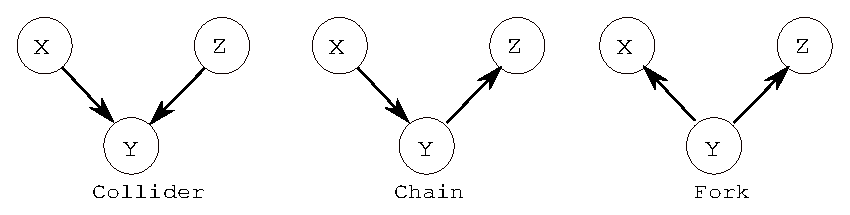
\includegraphics[width=0.70\textwidth]{vstructure.eps}
	\caption{Ternary conditional independence configurations}
	\label{fig:vstructure}
\end{figure}

Figure \ref{fig:vstructure} shows the three configurations which have the following conditional independence relationships; Chain : $X \ci Z | Y$, Fork : $X \ci Z | Y$, Collider: $X \ci Z$ but $X \dep Z | Y$. Of the three the collider that provides the so-called 'V-structure' is of most critical importance in causal discovery because it is the only configuration that provides unique causal characteristics of the three. Other configurations of three variables exist where the variables are not connected to each other, when they are connected in a cyclic manner and when they are fully connected with bi-directional arrows. These are of less interest here and are fully explored in separate branches of causal discovery.

It suffices to note that most algorithms in causal discovery aim at discovering V-structures in the data as a way of determining causal relationships in the data. Causal discovery methods have also been extended in several ways including; using bayesian networks to model causal relationships using conditional independencies, search-and-score methods of causal discovery, causal discovery in multivariate relatinoships between continous variables using Structural Equation Models (SEMs), causal discovery using Independent Componenet Analysis and more recently progress has also been in discovering causality from cause-effect pairs \cite{15,14}.

\section{RLVQ}
\label{sec:RLVQ}

The basic LVQ scheme is set up as follows; Given a dataset $D = \left\{x^\mu, y^\mu\right\}^P_{\mu = 1}$ where $x^\mu \in R^N$ and the labels $y^\mu \in {1,2,\ldots C}$ correspond to one of the classes, the LVQ scheme is parameterized by a set of prototype vectors $W = \left\{w_j, c(w_j)\right\}^M_{j=1}$ with the prototype vectors $w_j$ having labels $c(w_j) \in {1,2,\dots C}$.

For a particular dissimilarity/distance measure $d(x,w)$, the LVQ classifier employs a Winner-Takes-All scheme where an arbitrary input is assigned to the class $c(W_L)$ of the closest prototype with $d(x,W_L) \leq d(x,w_j)$ \textsl{for all} $j$.

LVQ was originally proposed by Kohonen and in the original heuristic formulation of LVQ, also called LVQ1\cite{02}, at each time step $t$ of an iterative training process, one example $\left\{x^\mu, y^\mu\right\}$ is selected randomly from the training set $(1 \leq \mu \leq P)$ and its distance $d(x^\mu,w_j(t))$  from all current prototypes $W$ is evaluated to obtain the closest(winner) prototype $w_j(t)$. This prototype is updated according to
%
\begin{align} 
w_j(t) = w_j(t) + \eta_w \phi (x^\mu - w_j(t)) \quad \text{with} \quad
\phi = \begin{cases}
+1& \text{if $y^\mu = c(w_j(t))$},\\
-1& else 
\end{cases}
\end{align}
%
The update is hence towards the actual introduced data point $\left\{x^\mu, y^\mu\right\}$ if the class labels of the data point and the winner agree or the update is away from the data point if the class labels disagree. The prototypes are initially placed close to the origin of the data with a small random offset.

In the literature, many modifications of Kohonen's original formulation have been suggested with the aim of achieving better convergence and generalization behavior. A specific set of modifications have been towards accounting for heterogeneous datasets where features can have different meanings and magnitudes. These are the class of relevance learning schemes which employ adaptive scaling factors for each dimension in the feature space. A good background to these modifications is given elsewhere in the literature\cite{09,10,11}. For our purposes it will suffice to give the general formulation of RLVQ.

For RLVQ we can consider a generalized Manhattan distance of the form
%
\begin{equation} 
d(x,w_j) = \sum^N_{j=1} \lambda_j (x_j - w_j)^2 ,
\end{equation}
%
as the dissimilarity measure where $\lambda_j$ are the adaptive relevance factors that are restricted to non-negative values and obey the normalization $sum^N_{j=1} \lambda_j = 1$. The special case $\lambda_j = 1/N$ for all $j = 1,\ldots N$ is analogous to the original LVQ1 formulation.

In line with equation (1), for each update of the winning prototype $w_j$ its corresponding relevance factors $\lambda_j(t)$ are updated as follows;
%
\begin{align}
\lambda_j(t) &= \lambda_j(t-1) - \eta_\lambda \phi (x_j - w_j)^2 \\
\lambda_j(t) &= \frac{max\left\{0,\lambda_j(t)\right\}}{\sum^N_{j=1} max\left\{0,\lambda_j(t)\right\}}
\end{align}
%
where equation (4) implements the non-negativity condition and the required normalization.

The $\lambda$ update hence decreases the relevance factor $\lambda_j$ if the winning prototype $w_j$ does represent the correct class but the contribution $|x_j - w_j|$ to $d(x,w_j)$ is relatively large. Conversely the weight of a feature with relatively small $|x_j - w_j|$ is increased in such a case. The learning rates $\eta_w$ and $\eta_\lambda$ control the magnitude of the prototype and relevance factor updates at each step.

Further simplifications of the RLVQ scheme to do inter-class or local relevance learning as opposed to the global learning scheme described herein have been implemented in the literature, however for our purposes here it suffices to use global relevances with the LVQ1 scheme as the simplest implementation of the relevance learning in prototype-based classification schemes. 

\section{CRLVQ}
\label{sec:CRLVQ}

The difference between RLVQ and CRLVQ is akin to the difference between correlation and causation. RLVQ outputs a relevance profile for the features that represents the importance of each feature for the classification task at hand. Generally the profile can also represent how correlated each feature is with the target. CRLVQ and causation on the other hand would ideally output features that have a causal effect on the target i.e. a change in the causes will cause a corresponding change in the target. If a new dataset is presented to the trained classifier in each of these cases, the RLVQ classifier is likely to give better performance is the data is of the same distribution as the training set. However if the distribution is different, CRLVQ is likely to give better performance to the degree to which the natural/former distribution has been intervened upon.

Our assessment of causal relevance is based on identifying V-structures with respect to the target. RLVQ gives a profile that represents how strongly each single dimension of the data is predictive of the target. In CRLVQ instead of looking at a single dimension, we look for evidence that there are two dimensions $x_i$ and $x_k$ that are predictive of the target. To ascertain that $x_i$ and $x_k$ are in a V-structure with the target we also check that they are independent of each other.

\begin{figure}
\begin{tabular}{m{.5\textwidth}cm{.4\textwidth}}
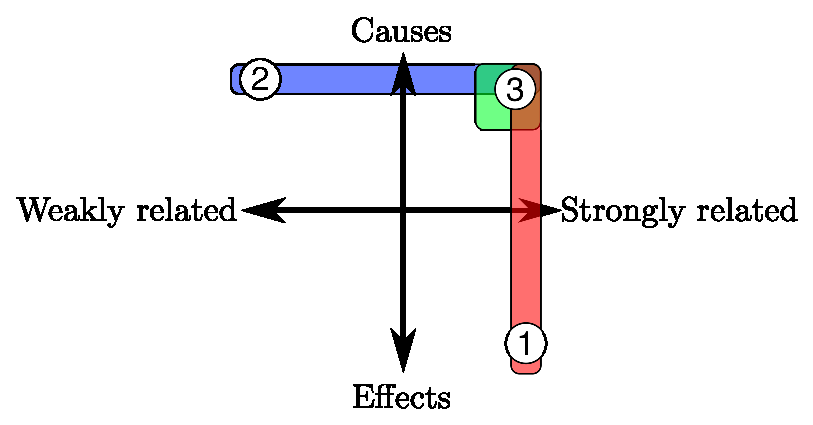
\includegraphics[width=.5\textwidth]{causal-relevance-dimensions.eps} & &
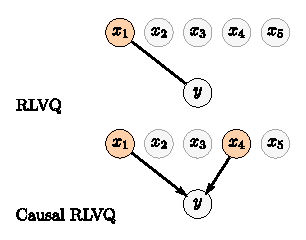
\includegraphics[width=.4\textwidth]{rlvq-crlvq.eps} \\
& \\
(a) & & (b)  
\end{tabular}
\label{fig:causes}
\caption{RLVQ and CRLVQ formulations. Panel (a) is an illustration of placement of variables across the predictive-causal space. Panel (b) shows how RLVQ is extended to CRLVQ}
\end{figure}

Figure 2 illustrates this salient distiction between RLVQ and CRLVQ. Panel (a) shows a placement grid for variables $(x_1, \ldots, x_P)$ categorised according to causal relevance or simply predictive relevance to the target variable $y$. Standard relevance learning aims to give higher weight to a set of variables (1) which are highly predictive; causal structure learning aims to find causes (2) or effects of a target; our work here identifies variables which are predictive causes (3). Panel (b) shows the criteria used for evaluating relevance scores in RLVQ and CRLVQ.

Through an iterative process, $\lambda$ the relevance vector in RLVQ is updated for each introduction of an example of the data based on the evidence the new example presents in support of how relevant each dimension is  for the prediction of the target. CRLVQ has two extra criteria to evaluate when updating the relevance vector. The three criteria in total are in a sense a distance-based formulation of the V-structure condition. Each component of $\lambda$ in CRLVQ is hence updated for every dimension $x_j$ for each introduction of a data example as follows
%
\begin{equation} 
\lambda_j(t) = \lambda_j(t-1) - \eta_\lambda \phi (x_j - w_j)^2 - \alpha \eta_\lambda \left( \min_{k \neq j}\left(\phi (x_k - w_k)^2 - (x_j - x_k)^2 \right) \right)
\end{equation}
%
The parameter $\alpha$ is a parameter that weights the two new criteria. Standard RLVQ is hence a special case of CRLVQ when $\alpha = 0$. We evaluate the independence of the different data dimensions by looking at their absolute difference. In z-transformed data, this will give a low number in the dimensions that are positively correlated. The update hence rewards any feature $x_j$ if it has a strong correlation(small distance apart) with the target/label vector $(|x_j - w_j|)$ , and also if there is strong evidence of another feature with a strong correlation to the target as well ($|x_k - w_k|$), and if feature $x_j$ and $x_k$ are weakly correlated (large distance apart).

Note however that there might be other relationships between the dimensions that make them dependent on each other, but that this update would not capture for example negative correlation. 

\section{Experiments}
\label{sec:Experiments}

Simulated causal networks were used to validate the causal $\lambda$ update. One causal network was formulated as a 4-feature linear Gaussian network with 2 causes and 2 effects. 

\begin{figure}
\begin{tabular}{cc}
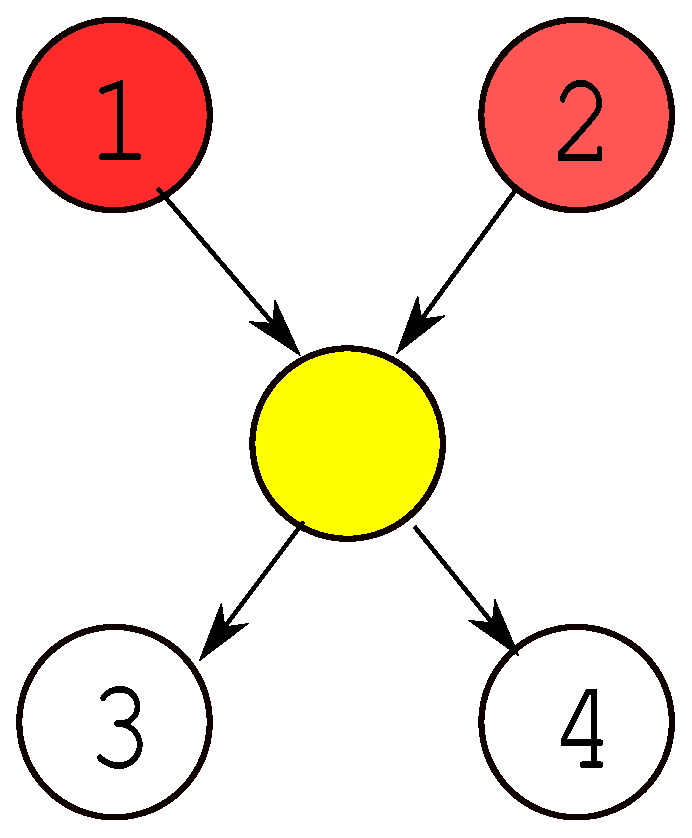
\includegraphics[scale=0.2]{simnetwork.eps} & 
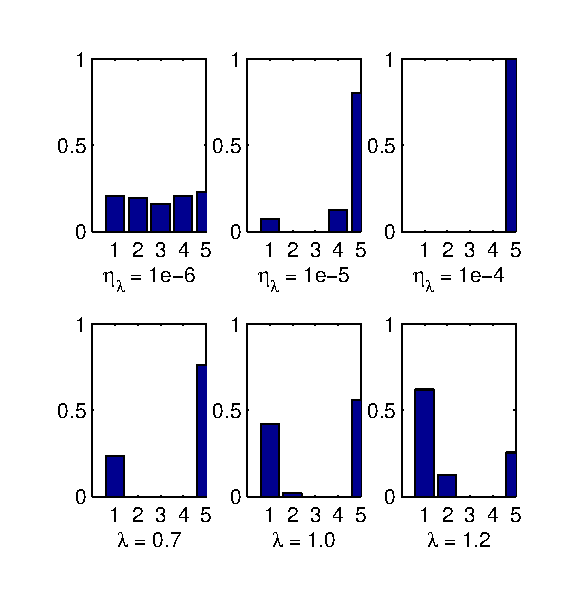
\includegraphics[width=.6\textwidth, height=.5\textwidth]{simlambda.eps} \\
(a) &  (b)  
\end{tabular}
\label{fig:simnetwork}
\caption{RLVQ and CRLVQ for Simulated Network. Panel (a) shows the simulated network with 2 causes and 2 effects. Panel (b) shows the relevance profile under RLVQ and under CRLVQ for different parameter settings.}
\end{figure}

From Figure 3, it is evident to see that with introduction of the causal update, the learning favours the features that are causally relevant over the 'just' correlated features. Making the learning rate for the causal update bigger results in bigger updates in the learning as well.

The second network was a network simulated from a Bayes net and used for several causal competitions as a trial set for tuning causal algorithms. It is commonly called the Lucas dataset\cite{12} and tries to predict lung cancer based on different features as shown in figure 2\\

\begin{figure}
\begin{tabular}{cc}
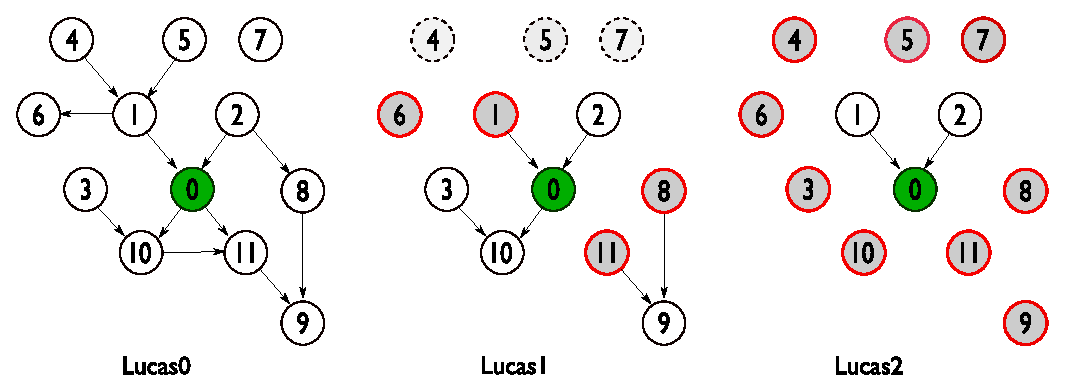
\includegraphics[width=.3\textwidth]{lucasgraph.eps} & 
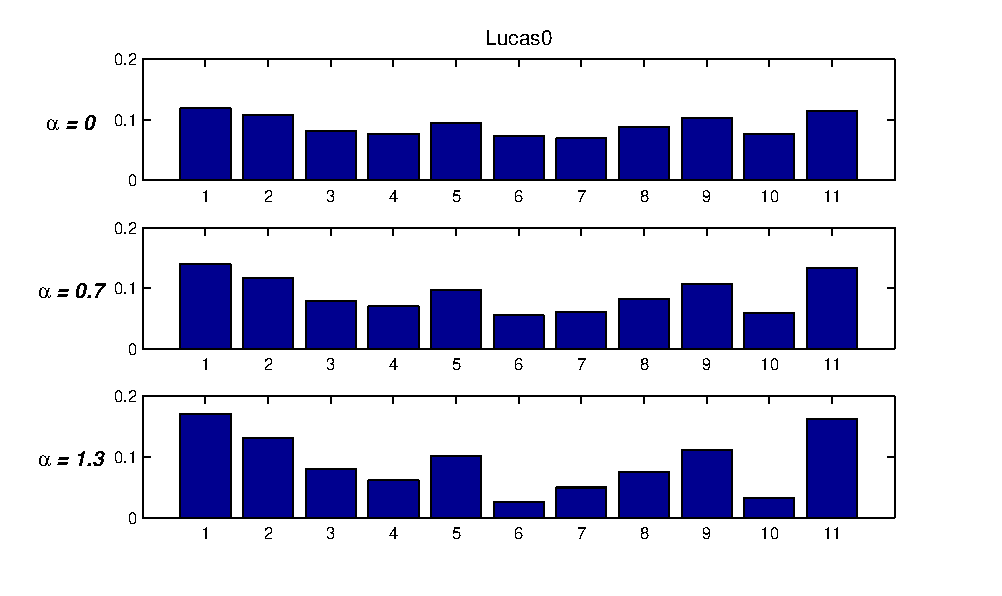
\includegraphics[width=.7\textwidth, height=0.6\textwidth]{lucaslambda.eps} \\
(a) &  (b)  
\end{tabular}
\label{fig:lucas}
\caption{RLVQ and CRLVQ for Lucas Network. Panel (a) shows the the lungcancer prediction (lucas) graph. Panel (b) shows the relevance profile under RLVQ and under CRLVQ for different parameter settings.}
\end{figure}

Figure 4 shows the influence of the causal update on a slightly more complicated network. The causal update tends to identify alot of the direct causes as $\alpha$ is increased. The peculiar nature of feature 10, being a direct cause of effect 11 as well as existing in a V-formation with features 3 and 0 is probably the reason why it appears as having causal relevance in the plots with $\alpha$ = 1e-4. For any larger values of $\alpha$ we obtain only one cause feature 1. Section \ref{sec:Results} gives the different performance based on these different relevance profiles.

To carry out experiments, we require a dataset with a training set from one distribution and test sets of the same dataset with different distributions. The easiest way is to manipulate the training set to get test sets of different distributions. A suitable set of datasets was obtained from the causality workbench datasets\cite{13}. A full description of the datasets and how they were manipulated can be found on the causality workbench site. We present a small description of the datasets for our purposes here.

\noindent
\textbf{REGED} - REsimulated Gene Expression Dataset; a gene expression dataset with 999 numeric features and split into 3 datasets, REGED0 - the natural unmanipulated dataset and REGED1 and REGED2 the same as REGED0 but with some variables manipulated or intervened on. Each of the 3 datasets has 500 examples.\\
\noindent
\textbf{CINA} - Census Is Not Adult; a marketing dataset derived from the UCI census adult dataset with 132 mixed variables and split into 3 datasets, CINA0 - unmanipulated natural dataset, CINA1 and CINA2 - manipulated datasets each with 16033 examples each.


\section{Results}
\label{sec:Results}

Table \ref{tab:TestErrorResults} shows the test error scores for the three datasets REGED, CINA and MARTI for CRLVQ with varying $\alpha$ parameters. The first row with $\alpha$ = 0 represents RLVQ. Set0 represents the unmanipulated(natural) dataset while sets 1 and 2 represent manipulated/intervened upon datasets. Test results are obtained after 50 epochs through the data with a constant learning rate for the prototypes for a particular dataset.


\begin{table}
	\centering
			\begin{footnotesize}
\begin{tabular}{|c|r|r|r|r|r|r|}
\hline
     CRLVQ &         \multicolumn{ 3}{|c|}{REGED} &          \multicolumn{ 3}{|c|}{CINA}  \\
\hline
$\alpha$ &     Set0 &       Set1 &       Set2 &       Set0 &       Set1 &       Set2 \\
\hline
  0    &     0.0400 &     0.0640 &     0.0640 &     0.1048 &     0.1018 &     0.1018 \\
\hline
  1e-6 &     0.0400 &     0.0640 &     0.0640 &     0.1484 &     0.1442 &     0.1442 \\
\hline
  1e-5 &     0.3600 &     0.2200 &     0.2200 &     0.1045 &     0.1047 &     0.1047  \\
\hline
  1e-4 &     0.3900 &     0.0420 &     0.0420 &     0.0945 &     0.0955 &     0.0955  \\
\hline
  1e-2 &     0.8900 &     0.8820 &     0.8820 &     0.0970 &     0.0876 &     0.0876  \\
\hline
\end{tabular}   
			\end{footnotesize}
	\caption{Test Error results for RLVQ and CRLVQ for the different datasets REGED and CINA.}
	\label{tab:TestErrorResults}
\end{table}

It is interesting to note that for the unmanipulated set (column Set0), the performance generally degrades as you tune the parameter from RLVQ towards CRLVQ. This is plausible because for high values of $\alpha$, CRLVQ gains more sensitivity and hence filters out more false causes(e.g. effects) which would potentially be relevant for classification hence degrading the performance. For the cina dataset this is not necessarily true. It is possible that cina would behave differently because it has a comparatively lower dimension (132 vs 999) and more examples (16033 vs 500)

Performance as the value of $\alpha$ increases again generally seems to get better for the manipulated sets 1 and 2 than performance with the RLVQ classifier. This again seems plausible because causes identified by CRLVQ remain predictive even when the data is intervened upon while the relevant features identified by RLVQ may not necessarily remain predictive in the same situation. At even higher values of $\alpha$ for the Reged dataset with high dimensionality and few examples, performance starts to degrade. It is possible that a very big $\alpha$ will produce a narrower set of relevant features that not sufficiently model the data for the classification problem at hand.

Similar results are obtained for sets 1 and 2 for all datasets. For CRLVQ this is plausible because it identifies causes which remain predictive no matter what interventions the data goes through. So for differently intervened upon datasets of the same natural datasets, CRLVQ would probably classify the same since the causes remain the same in the different instances of the data. However the fact that RLVQ also gives the same results for the manipulated sets could mean that the manipulations between the two sets were not significant enough to warrant a big disparity in the test error.

\section{Conclusion}
\label{sec:Conclusion}

This paper attempts to leverage techniques in causal learning and discovery and apply them to relevance learning for prototype-based classification. The goal is to assure robust classification when it is not certain that the test set has the same distribution as the training set, which is a common scenario in real applications. While our scheme is theoretically plausible, its actual formulation is still not very specific. This paper attempts a possible proof of concept and as such has several limitations in its present formulation; for example the scheme will only work if there are more than one cause and the causes are not related to each other. Also if causative cycles are present in the data, unreliable performance will result. 

The introduction of $\alpha$ is interesting because it can be tuned across a scale of RLVQ to CRLVQ and in a sense can depict the degree of certainty of manipulation of the test set. Presently this parameter is set arbitrarily, future work will look into how to learn this parameter as well. We also used a basic derivative of LVQ which has inherent problems in convergence and generalization of the classifier, however since CRLVQ mainly is about how to update the relevance vector, we believe it can be easily extended to the different derivatives of LVQ including GRLVQ, GMLVQ and others. In future we will attempt to extend the update to these different schemes as well. Our formulation of the V-structures is not very specific and we have tried to highlight the short comings in different sections of this paper, in future providing a proper formulation will be one of our key concerns.

% ****************************************************************************
% BIBLIOGRAPHY AREA
% ****************************************************************************

\begin{footnotesize}

\bibliographystyle{unsrt}
\bibliography{esann2011}

\end{footnotesize}

% ****************************************************************************
% END OF BIBLIOGRAPHY AREA
% ****************************************************************************

\end{document}
